%  con su pequeno parrafo intruductorio para cada uno
\chapter{Desarrollo de la metodología de la investigación}
\section{Diagrama de flujo}
El diagrama de flujo de la metodología de la investigación proporciona una representación visual de los pasos secuenciales seguidos durante el desarrollo del proyecto \cite{Clark2026}. Este diagrama detalla desde la identificación del problema hasta la validación del prototipo, facilitando la comprensión de las etapas del proceso.
% agregar el diagrama de flujo de la metodología de la investigación
\begin{figure}[H]
    \centering
    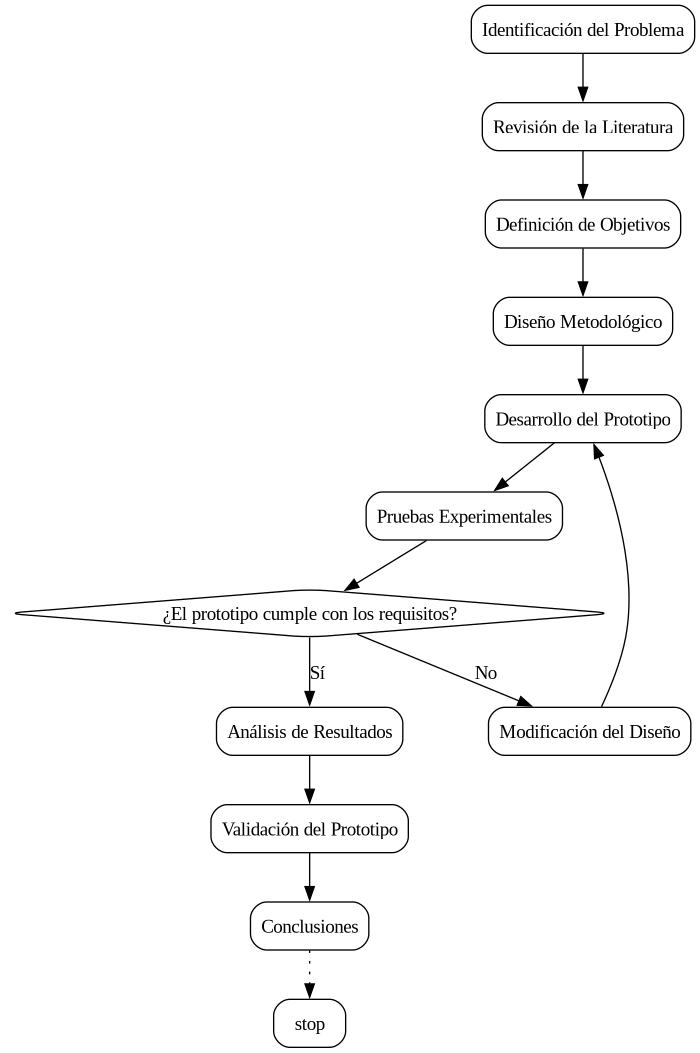
\includegraphics[width=1\textwidth]{img/Metodologia.png}
    \caption{Diagrama de flujo de la metodología de la investigación.}
    \label{fig:flowchart}
\end{figure}


\section{Diagrama de proceso}
El diagrama de proceso detalla las actividades principales involucradas en el desarrollo del exoesqueleto, desde el diseño conceptual hasta la prueba y validación con usuarios. Este diagrama muestra el flujo de actividades, entradas y salidas, proporcionando una vista clara del enfoque estructurado adoptado en la investigación.
% agregar el diagrama de proceso de la metodología de la investigación
\begin{figure}[H]
    \centering
    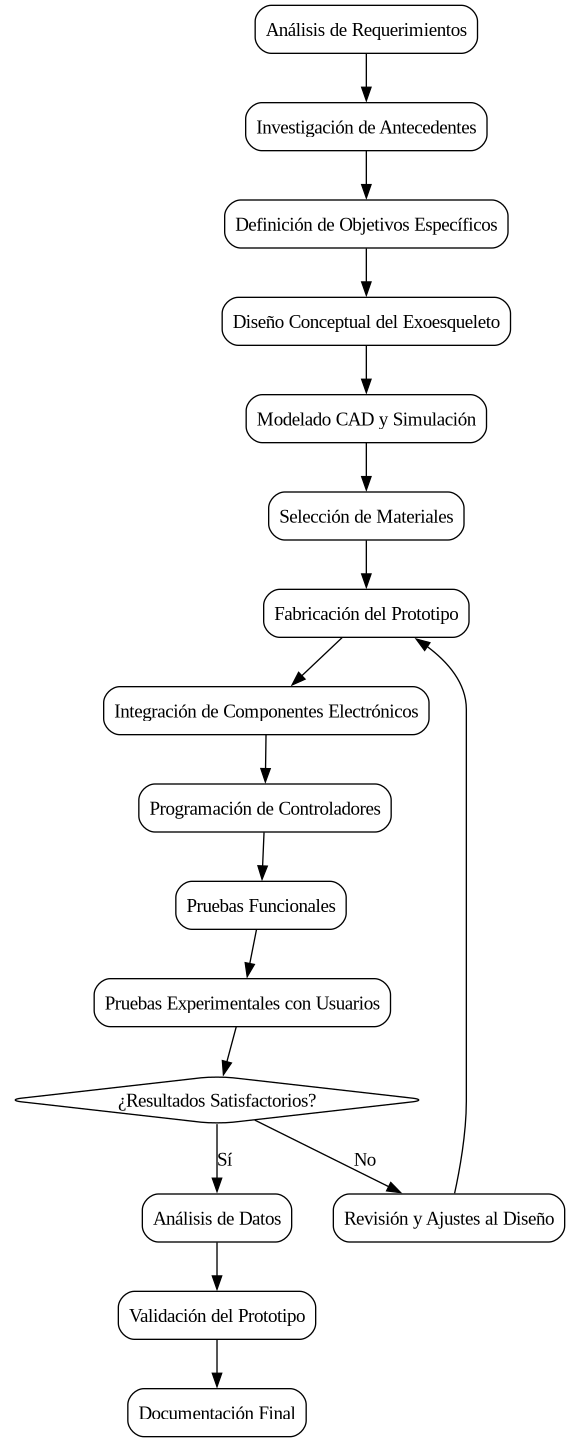
\includegraphics[width=0.6\textwidth]{img/Proceso.png}
    \caption{Diagrama de proceso del desarrollo del exoesqueleto.}
    \label{fig:flowchart}
\end{figure}

\section{Diagrama de bloque}
El diagrama de bloque simplifica los componentes clave del sistema desarrollado, identificando los módulos principales y su interacción. Este diagrama proporciona una vista de alto nivel de la arquitectura del exoesqueleto y cómo se integran sus diferentes partes.
% agregar el diagrama de bloque de la metodología de la investigación (este dijo raquel que nos lo iba a explicar pero no se si le alcanze el tiempo)
\begin{figure}[H]
    \centering
    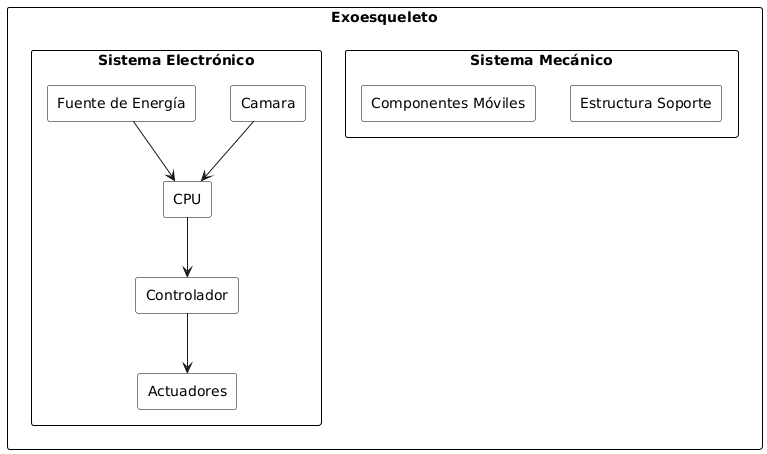
\includegraphics[width=1\textwidth]{img/DiagramaBloque.png}
    \caption{Diagrama de bloque del exoesqueleto prototipado.}
    \label{fig:flowchart}
\end{figure}